\documentclass{beamer}
\usepackage{style}

\title{M05 - Mini project}
\subtitle{Human Activity Recognition from Continuous Ambient Sensor Data}
\author{Steve Devènes, Amara Spano}
\institute{Unidistance}
\date{\today}
\usetheme{Madrid}

\begin{document}

	\begin{frame}
		\titlepage
	\end{frame}

	% \begin{frame}
	% 	\frametitle{Outline}
	% 	\tableofcontents
	% \end{frame}

%	\begin{frame}
%		\frametitle{Selected project}
%	\end{frame}

	\begin{frame}
		\frametitle{Working hypothesis}
		It's possible to perform human activity recognition from continuous ambient sensor data.
	\end{frame}

	\begin{frame}
		\frametitle{Data}
		Data is available online on the UC Irvine machine learning repository.

		Data are downloaded automatically.

		The dataset is large, it contains 36 features measured plus one output for the classification label
		of the activity (35 differents activities), for a total of 13956534 entries.

		There are two evaluation protocols:
		\begin{figure}
			\centering
			%\includegraphics[width=\linewidth]{idiap_web.jpg}
			\missingfigure{Protocols illustration}
		\end{figure}
	\end{frame}

	\begin{frame}
		\frametitle{Workflow}
		For different experiments:
		\begin{enumerate}
			\item Load the training data
			\item Create and train a random forest classifier
			\item Load the test data
			\item Make prediction on test data
			\item Print the confusion matrix for the model evaluation. Confusion matrices are also available in graphs with plotly.express.
		\end{enumerate}

		The experiments run sequentially.
	\end{frame}

	\begin{frame}
		\frametitle{Version control}
		On github at \url{https://github.com/sdevenes/M05_MiniProject}

		The work is organized using github issues to create and assign tasks.

		The general approach:
		\begin{itemize}
			\item Create 1 branch per feature named \textit{feature/feature\_name}
			\item When the feature is complete, do a pull request with the other as a reviewer
		\end{itemize}

		\begin{figure}
			\centering
			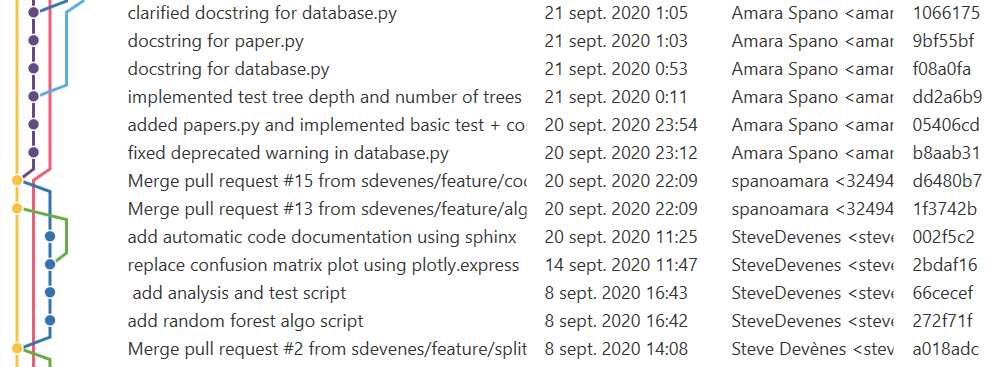
\includegraphics[width=\linewidth]{img/git_tree.png}
		\end{figure}
	\end{frame}

%	\begin{frame}
%		\frametitle{Version control}
%		\begin{figure}
%			\centering
%			%\includegraphics[width=\linewidth]{idiap_web.jpg}
%			\missingfigure{Git tree illustration}
%		\end{figure}
%	\end{frame}

	\begin{frame}
		\frametitle{Unit Testing and CI}
		The majority of the functions in the code are covered by unit-tests,
		this was done using Nose python package.
		(percentage of coverage ?)

		These tests are run at each commit through travis CI:
		\url{https://travis-ci.org/github/sdevenes/M05_MiniProject}
		Procuring a quick detection of bugs and errors that could appears
		during the project development.
	\end{frame}

	\begin{frame}
		\frametitle{Documentation}
		Each function is commented with a docstring. The documentation is
		then build automatically in the CI using Sphinx at each new commit on the
		master branch.

		Doc available here: \url{https://sdevenes.github.io/M05_MiniProject/index.html}
	\end{frame}

	\begin{frame}
		\frametitle{Packaging and Deployment}
		To do
	\end{frame}

%	\begin{frame}
%		\frametitle{Final remarks}
%	\end{frame}
\end{document}
